
% We now discuss \oak's data organization.
\oak\ allocates keys and values off-heap and metadata on-heap, as described in \Cref{ssec:on-off}.
 \Cref{ssec:mm} presents \oak's simple internal memory manager, which  controls off-heap allocation and garbage collection.
To allow user code safe access to data in \oak\/ buffers without worrying about concurrent access 
or dynamic reallocation,  \oak\ employs an  indirection layer called \emph{handle}, as discussed in \Cref{ssec:handles}. 

\subsection{Off-heap data and on-heap metadata}
\label{ssec:on-off} 

\begin{figure*}[tb]
\setlength\belowcaptionskip{0pt}
\setlength\abovecaptionskip{0pt}
\begin{subfigure}{0.4\linewidth}
\centering
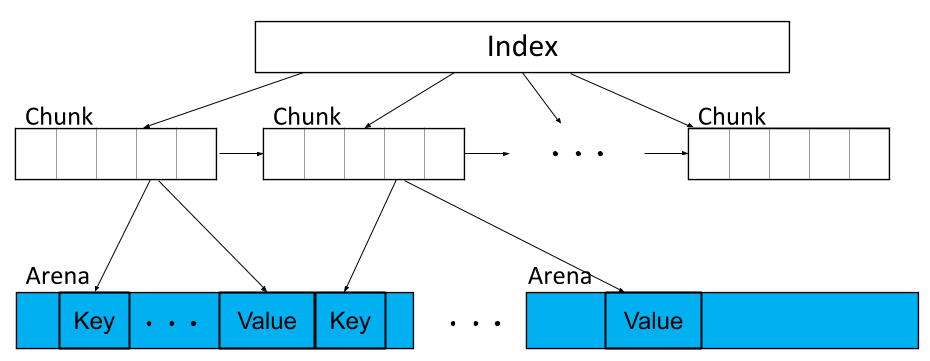
\includegraphics[width=\textwidth]{layout.png}
\caption{Index, chunks, and arenas}
%: the index and chunk list are on heap, whereas keys and values are allocated in off-heap arenas.
\label{fig:index}
\end{subfigure}
\hfill
\begin{subfigure}{0.515\linewidth}
\centering
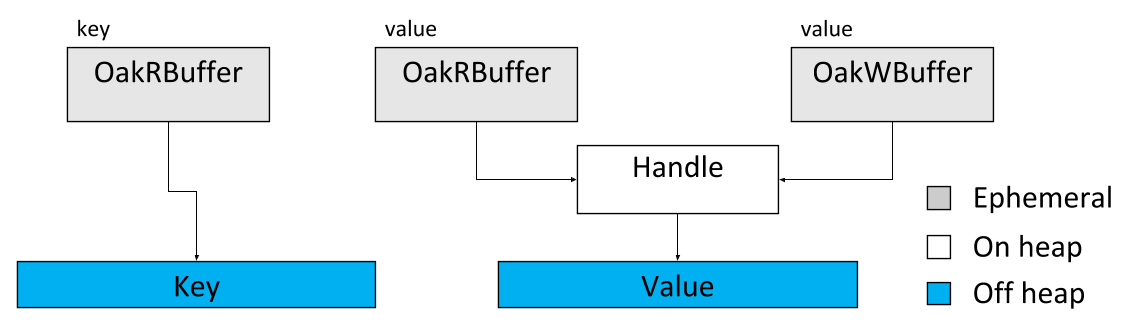
\includegraphics[width=\textwidth]{handle.png}
\caption{Buffers, handles, and data}
\label{fig:handle}
\end{subfigure}
\caption{\oak\ data organization.}
\end{figure*}

% \paragraph{Chunks and index.} 
Oak's on-heap metadata maps keys to values. It
is organized as a linked list of \emph{chunks} -- large blocks of contiguous key ranges, as  in \cite{chunks}. 
Each chunk has a \emph{minKey}, which is invariant throughout its lifespan.
We say that key $k$ is in the \emph{range of chunk $C$} if $k \geq C.$\emph{minKey} and $k < C.next.$\emph{minKey}.

A chunk includes a linked list of \emph{entries},  
%organized as an array-based linked list, 
sorted in ascending key order. 
The entries point to off-heap keys and values. 
%Each entry holds 
%(1) a pointer to a key (off-heap), 
%(2) a pointer to a handle (in the same chunk, on-heap) that points to an off-heap value, 
%and the index of the entry that holds the next key in the linked list. 
\oak\ makes sure that each key appears in at most one entry.


To allow fast access, we follow the approach of \cite{the-art-of,index-1,index-2,kiwi,transactional-lib} and add an \textit{index} 
that maps minKeys to their respective chunks, as illustrated in \Cref{fig:index}. %Each chunk is indexed according to its minKey. 
The index %offers standard lookup, insert, and remove operations. It
is updated in a lazy manner, and so it may be inaccurate, in which case, locating a chunk may involve a partial 
traversal of the chunk linked list. % (as in \cite{kiwi}). 
A \algvar{locateChunk(k)} method returns the chunk whose range includes  key \algvar{k} by querying the index and traversing the chunk list if needed. 

%\paragraph{Intra-chunk organization.}
% As shown in Figure~\ref{fig:chunk}, chunks hold three types of objects: entries, keys, and handles. 



%Given that the prefix and the remainder are of similar sizes, the expected search time remains polylogarithmic. 
%Nevertheless, in the worst-case, the search time is linear in the size of the remainder of the chunk. 

\remove{
\begin{figure}
\centering
\includegraphics[scale=0.4]{chunk.png}
\caption{Oak intra-chunk organization.}
\label{fig:chunk}
\end{figure}
}

\subsection{Memory management}
\label{ssec:mm} 

\oak\ offers a simple default memory manager  that can be overridden by applications.
The default manager  is suitable for real-time analytics settings, where  
dynamic data structures  used to ingest new data  exist for limited time~\cite{Druid,hbase} and
%The operations are mostly inserts and in-situ updates, while 
deletions are infrequent.
%, which motivates the following simple design.  

%Memory management involves two aspects -- {allocation} and GC. 
\oak's allocator manages a shared pool 
of large  (100MB by default) pre-allocated off-heap {\em arenas}, and supports multiple \oak\ instances.  
Each arena is associated with a single \oak\/ instance and returns to the pool when that instance is disposed. 
{Key and value buffers  are allocated from the arena's flat free list 
using a  first-fit approach; they  return to the free list upon KV-pair deletion %(\cref{ssec:handles}) 
or value resize.}

The memory manager can efficiently compute the total size of an \oak\ instance's  off-heap footprint.
%as required by some applications~\cite{HbaseSizeTracking}.


\subsection{Handles and  concurrency control}
\label{ssec:handles}

The handle abstraction provides access to off-heap mutable memory, bridging between the on- and  off-heap parts of \oak,  
as shown in \Cref{fig:handle}. There is a single handle per value, which the  
\algvar{OakRBuffer} and \algvar{OakWBuffer} objects  wrap. Keys are immutable, so their 
\algvar{OakRBuffer}s reference off-heap memory directly, without handles.  
%
Since the handle is an on-heap object, it remains reachable to  threads that hold \oak\ buffers that wrap it 
 after the value  (off-heap) is reclaimed. 



%The handle has the same interface as a Java ByteBuffer, as do the values, which makes them amenable to off-heap allocation. 
The handle ensures that all methods are applied to the buffers atomically. 
The default implementation uses a read-write lock, but can be overridden, e.g., by an optimistic approach.
The handle also interacts with the memory manager in order to dynamically resize values
(requesting a new allocation and copying the buffer to it if needed), 
and informs it when to reclaim buffers that are no longer needed.
%The memory manager is a separate module and is also replaceable.

Once a value is removed from Oak, the handle assures that no thread will attempt to read it, since 
that memory may be reclaimed. 
To this end, the handle performs a logical remove by marking itself as deleted.
A key is deemed present in Oak only if it is associated with a non-deleted handle.
%All other handle operations check if the handle is deleted before taking any action.
% 
The handle further offers 
update and compute mechanisms that are used by \oak\/ to atomically modify values.
%The former directs the handle to  reference to the given value, whereas the latter executes a user-provided lambda, while ensuring that the update occurs 

